\begin{surferIntroPage}{SURFER 시작하기}{tutorial_koord1}{SURFER 시작하기}
이 프로그램은 SURFER 라고 합니다. 이 단어를 보시면 아마 여러분은 물, 태양 그리고 파도를 떠올리실 겁니다. 하지만 이 단어는 {\it surface} 라는 단어에서 유래하였습니다.
\\
SURFER를 이용하여 우리는 표면(surface), 좀더 정확하게는 대수곡면을 표현할 수 있습니다. 이게 무슨 말인지 그리고 대수곡면이 무엇인지는 이 튜토리얼에 설명되어 있습니다. 옆의 그림을 선택하여 학습해 나가십시오.\\
SURFER는 2008 독일 수학의 해에 시작된 이동형 전시관인 IMAGINARY의 일부입니다. IMAGINARY는 독일 남서부 삼림지대에 있는 Mathematisches Forschungsinstitut Oberwolfach에 의해 기획되었습니다. 연구소에서는 매주 최신 수학을 주제로 워크숍이 열립니다. 이 워크숍들은 전세계의 수학자의 교류를 활성화 시키는 데에 굉장히 중요한 역할을 합니다.\\
\vspace{0.2cm} \hspace{3.5cm}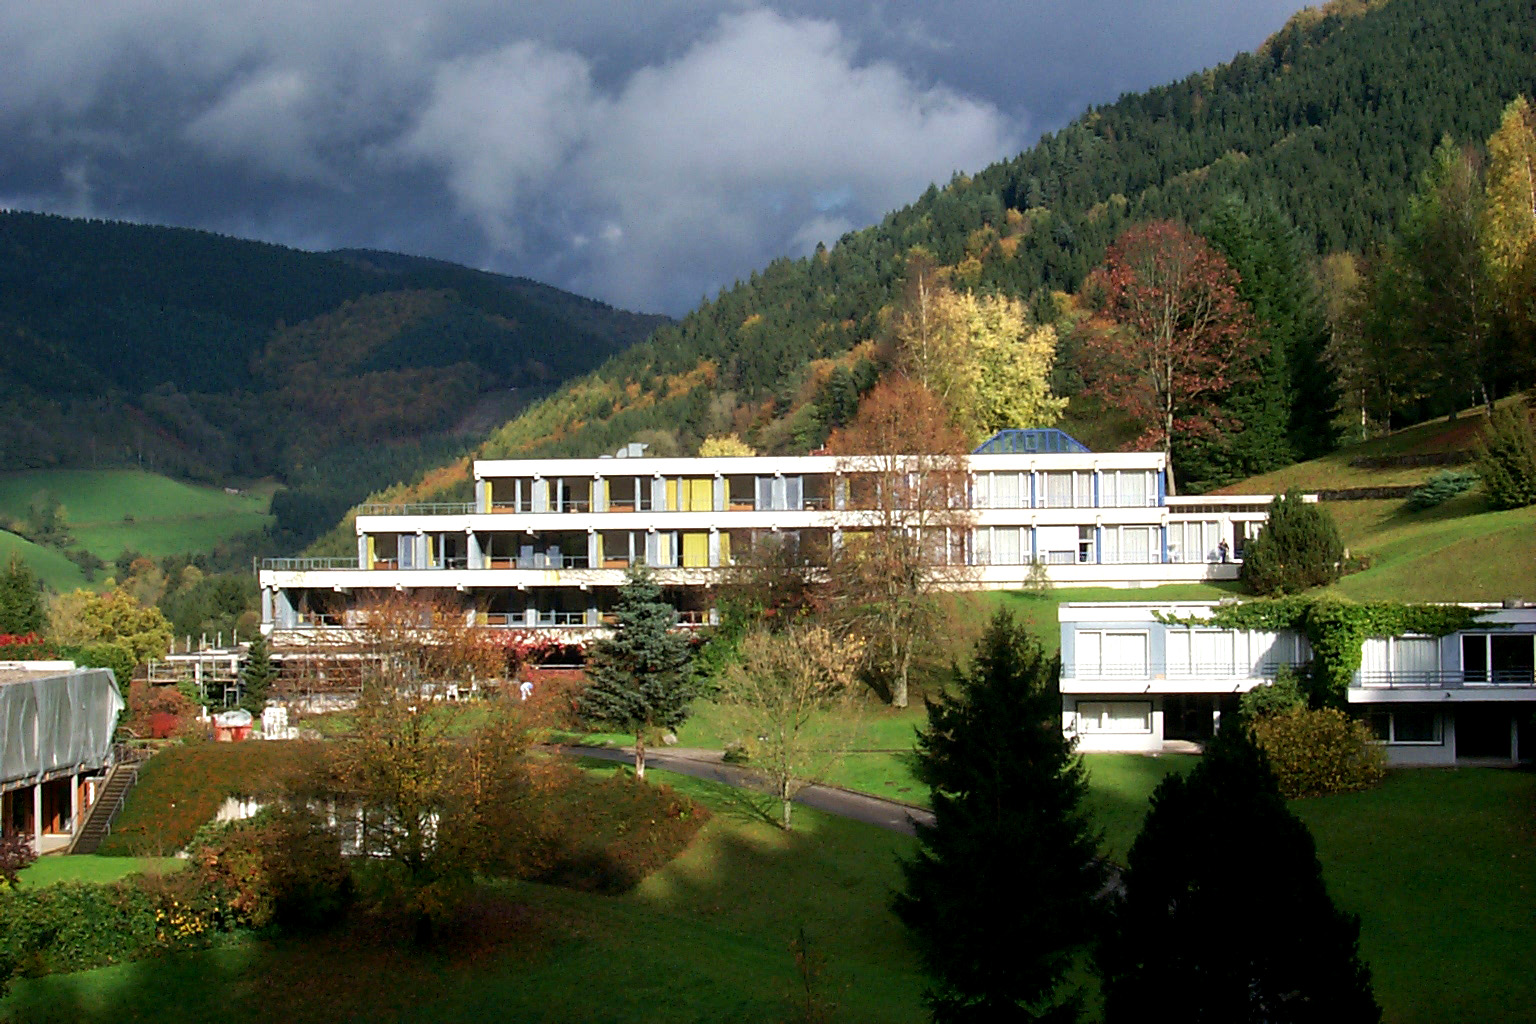
\includegraphics[width=3cm]{./../../common/images/photo_mfo.jpg}\\
이 프로그램은 다음의 웹사이트에서 다운받을 수 있습니다.: \\
\begin{centering}
www.imaginary-exhibition.com\\
\end{centering}
 \vspace{0.2cm}
오른쪽에서 여러분은 Zitrus 부터 시작하는 수학 튜토리얼 선택할 수 있습니다. 왼쪽에서는 fantasy surafaces 같은 다른 갤러리로 이동할 수 있습니다.
\end{surferIntroPage}
